\section{Mjukvaruarkitektur}

Arkitekturen utformades utgående från samma principer som den tekniska arkitekturen. Systemet har planerats utgående ifrån skalbarhet. Det vill säga att systemet skall vara lätt att utveckla funktionsmässigt, det skall vara lätt att underhålla systemet och det skall vara lätt att öka dess kapacitet vid behov. \citep[s. 203]{scalableweb}

\subsection{Horisontell skalbarhet}

För att tillåta systemet att anpassas till växande resurskrav, har SmartElement utformats för att tillåta horisontell skalbarhet. Att ett system är horisontellt skalbart betyder att man kan öka systemets kapacitet genom att öka antalet av någon komponent och sprida ut belastningen. \citep[s. 205-207]{scalableweb}

I SmartElements fall betydde det att mjukvaruarkitekturen måste vara tillräckligt flexibel för att kunna köras på flera servrar. Detta ledde till en modulär design som försöker separera ansvarsområden inom mjukvaran. På så vis kan de olika delarna byggas ut oberoende av varandra.

Den tyngsta delen av applikationen, vad gäller skalbarhet, är applikationsdatabasen. På grund av detta skapades processer som är menade att skydda detta lager genom att spara objekt i cache-minnet. På så vis hålls databasförfrågningarnas antal lägre och applikationsdatabasen behöver inte vara lika skalbar för att systemet skall klara större mängder förfrågningar.

\subsection{Servern}

\begin{figure}[h!]
\centering
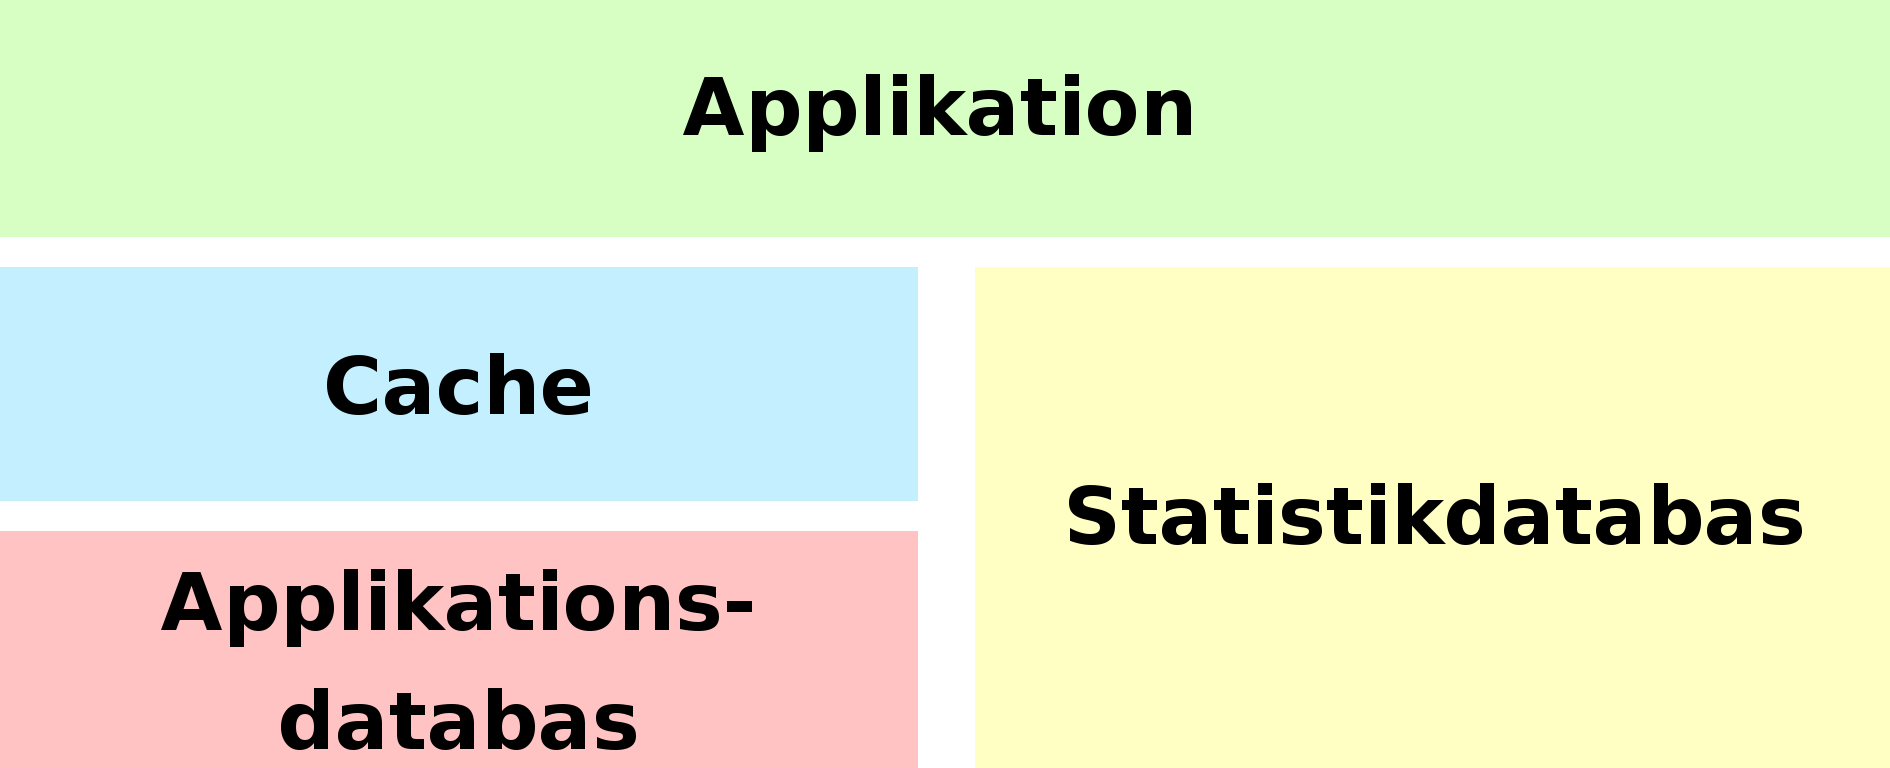
\includegraphics[width=120mm]{assets/images/smelementbackendparts.png}
\caption{Serverkomponentens delar}
\label{abstractbackend}
\end{figure}

Back-endsystemet, dvs. serverkomponenten, i SmartElement är den centrala delen av systemet var all data lagras och all filtrering sker. De delar som bygger upp serverkomponenten illustreras i Figur \ref{abstractbackend}. Systemet har två gränssnitt, ett öppet som används av tagen för att hämta innehåll vid sidvisningar, och ett stängt som används av en frontend vid konfiguration.

Hela back-endsystemet är realiserat med en fokus på att vara tillståndslöst (jmfr. engelskans \textit{''stateless''}) vad gäller hanteringen av förfrågningar. I praktiken betyder detta att man inte skall behöva en session med back-enden för att kunna genomföra förfrågningar, utan all information som behövs förses antingen i förfrågningen, eller så kan den generaras från databasen. Detta betyder att t.ex. autentiseringen är baserad på en nyckel som används för att generera en signatur för varje förfrågning. Orsaken till detta ligger i att det är lättare att realisera horisontellt skalbarhet i systemet genom att lägga till applikationsservrar, då sessioner inte behöver synkroniseras mellan de olika servrarna.

Tekniskt sett så finns det fyra huvudsakliga komponenter i back-endsystemet: applikationen, cache-lagret, applikations-databasen och statistik-databasen. Denna uppdelning är gjord för att försöka tillåta för oberoende horisontell skalbarhet i de olika ansvarsområdena genom att lägga till eller ta bort resurser av de olika komponenterna i takt med behov.

\subsection{PHP-ramverket Laravel}

För att göra utvecklingen av systemet snabbare användes ett utvecklingsramverk. Ett utvecklingsramverk är en samling av kodpaket som används som bas vid utvecklingen av en applikation och förser utvecklaren med funktionalitet som inte varierar mycket mellan applikationer.

Ramverket som används för att utveckla SmartElement är PHP-ramverket Laravel. Det är ett yngre ramverk som utvecklats med komponenter från Symfony-ramverket, ett väletablerat PHP-ramverk som dock kan vara rätt tungt. Laravel drar även full nytta av pakethanteraren Composer, vilket tillåter lätt importering av kodpaket i projektet. Utöver detta är hela ramverket uppbyggt för att vara modulärt och tillåter således modifikation eller full ersättning av komponenter.

Laravel-ramverket bygger på mönstret \gls{mvc} i sin arkitektur. Dvs. att ramverket delar upp ansvar i olika komponenter: datalager (Model), presentationslager (View) och kontrolllager (Controller). Datalagret ansvarar för applikationslogik och data, presentationslagret ansvarar för att presentera data och kontrolllagret ansvarar för att binda ihop presentations- och datalagret.\citep[s. 14-16]{gof}

\subsection{Komponenter i systemet}

SmartElement består egentligen av endast några få centrala komponenter som tillsammans skapar delarna i identifikation av besökare och filtrering av innehåll. Här beskrivs dessa centrala komponenter och deras egenskaper.

\subsubsection{Sidvisningshanteraren}

Den centrala delen av hanteringen av en sidvisning sker i en hanterare som tar emot information om besökaren och söker fram det innehåll som skall skickas tillbaka. Rent tekniskt så tar denna komponent emot en förfrågning från besökarens webbläsare, synkroniserar informationen med statistikdatabasen, söker fram sidobjektet ur cachinglagret (alternativt bygger upp det från databasen), använder siteobjektet för att generera det innehåll som skall sändas tillbaka och formaterar ett svar som skickas tillbaka till besökaren.

\subsubsection{Besökarobjektet}

\begin{figure}[h!]
\centering
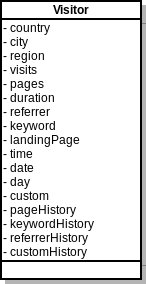
\includegraphics[width=40mm]{assets/images/umlVisitor.png}
\caption{Besökarobjektet}
\label{visitoruml}
\end{figure}

Besökarobjektet, illustrerat i Figur \ref{visitoruml}, representerar en besökare på webbsidan och innehåller all information som systemet kunnat samla ihop. Besökarobjektet är det enda objekt i filtreringsprocessen som är realiserat att använda databasen.

När en förfrågan kommer in, anropas en metod som försöker hitta besökaren i statistikdatabasen. Om ett resultat hittas, uppdaterars det befintliga objektet med den nya informationen från förfrågningen. Om besökaren inte är igenkänd så skapas ett nytt besökarobjekt med den försedda informationen.

\subsubsection{Siteobjektet}

\begin{figure}[h!]
\centering
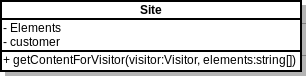
\includegraphics[width=90mm]{assets/images/umlSite.png}
\caption{Siteobjektet}
\label{siteuml}
\end{figure}

Sitebjektet, illustrerat i Figur \ref{siteuml}, är det högsta objektet i hierarkin som används för att filtrera ut innehåll. Det beskriver upprätthållarens webbplats i sin helhet. Från sitebjektet går alla relationer hela vägen ner till filtren som används för att välja ut innehåll.

När sidvisningshanteraren samlar ihop data för att skicka tillbaka till besökaren så anropar den siteobjektet med ett besökarobjekt. Därefter sköter siteobjektet om att anropa de olika elementen som sparats under sidan och ber dessa filtrera ut lämpligt innehåll innan det lämnar tillbaka kontrollen till sidvisningshanteraren.

Objektet är realiserat så att det kan kompileras till en entitet som går att spara i ett cache-lager för kunna hålla objektet i minne vid operationer. Detta tillåter snabb åtkomst till data under en sidvisning och sparar på databasförfrågningar.

\subsubsection{Elementobjektet}

\begin{figure}[h!]
\centering
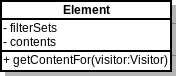
\includegraphics[width=40mm]{assets/images/umlElement.png}
\caption{Elementobjektet}
\label{elementuml}
\end{figure}

Elementobjektet, illustrerat i Figur \ref{elementuml}, motsvarar ett HTML-element på användarens webbplats, men det är ej bundet till någon specifik webbadress eller sida på webbplatsen. Detta betyder att man kan använda samma element på olika sidor under samma webbplats om man vill, t.ex. i en banner eller som del av en navigation.

\subsubsection{FilterSetobjektet}

\begin{figure}[h!]
\centering
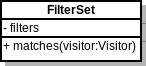
\includegraphics[width=40mm]{assets/images/umlFilterSet.png}
\caption{FilterSetobjektet}
\label{filtersetuml}
\end{figure}

Ett element innehåller filterset, innehåll och ett status. Figur \ref{filtersetuml} representerar ett FilterSetobjekt. Filterseten är filtersamlingar med en länk till ett innehållsobjekt samt en prioritet inom elementet. När sidobjektet anropar ett element för att få tillbaka det lämpliga innehållet kör elementet igenom sin filtersetsamling och ser om filtren passar besökarobjektet. Om fler en ett filterset passar så väljs det med högsta prioritet. När ett filterset valts ut så returnerar elementet det innehåll som filtersetet är länkat till. Om inget filterset passar så returneras ett tomt resultat.

Filterseten bygger tillsammans med filtren på ett utvecklingsmönster som kallas för ''Strategy pattern''. Idén är att man genom att definiera ett bra gränssnitt för en process, lämnar systemet öppet för enkel vidareutveckling i ett senare skede. \citep[s. 349]{gof} FilterSetobjektet i samband med besökarobjektet utgör tillsammans det sammanhang i vilket strategierna (Filtren) appliceras.

\subsubsection{Filterobjektet}

\begin{figure}[h!]
\centering
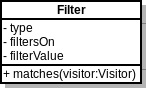
\includegraphics[width=40mm]{assets/images/umlFilter.png}
\caption{Filterobjektet}
\label{filteruml}
\end{figure}

Filterobjekten är i slutändan de objekt som utför tester mot besökarobjekten. Som Figur \ref{filteruml} illustrerar består de av en filtertyp som definierar hur de jämför data, en fältidentitet som de använder för att läsa ut data ur besökarobjektet, ett värde som de testar mot och ett villkor som de använder för att utföra testet.

Filterobjekten implementerar strategin i filtreringen som utförs i samband med filterseten. Ett filter tar endast ställning till en sak och returnerar ett logiskt värde beroende på om kriteriet möts eller ej. Filtersetet vet endast att det kan innehålla godtyckligt filter och filtret i sig vet att frågan alltid kommer att ställas på samma vis med likadan input.

\subsubsection{Contentobjekten}

\begin{figure}[h!]
\centering
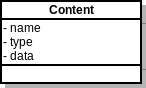
\includegraphics[scale=1]{assets/images/umlContent.png}
\caption{Contentobjektet}
\label{contenttuml}
\end{figure}

Contentobjektet, illustrerat i Figur \ref{contenttuml}, är den data som returneras till besökaren efter att filtreringen skett. Systemet sätter ingen annan begränsning på datan än att den måste kunna sparas som en textsträng. Detta betyder att man kan producera avancerad funktionalitet genom att t.ex. spara Javascript-kod eller \gls{json}-data som innehåll och på så vis använda SmartElement för att styra exekvering i besökarens webbläsare. Det betyder också att systemet inte sätter så stora krav på anroparen eftersom det enda som är viktigt är att denne kan tolka datan som returneras. Detta betyder att man i princip kunde skapa godtycklig klient till back-enden genom att implementera protokollet som tagen använder.

\subsection{JavaScript-tagen}

JavaScript-tagen är en kort kod som laddas i samband med webbsidan och samlar ihop information om besökaren och sedan skickar denna information till back-endsystemet för processering.

Tagen försöker hitta en s.k. kaka i besökarens webbläsare. Om ingen finns så skapas en ny unik id som sparas i en ny kaka. Efter att tagen fått en id, läser den ut information från besökarens webbläsare. Den läser bl.a. hänvisarinformationen och extraherar sökord om hänvisaren varit en sökmotor. Tagen kan även räkna ut tiden för besöket med hjälp av en tid som sparas i kakan då den skapas. Om sidvisningen är den första i besöket läser tagen adressfältet och använder värdet som landningssida för besöket. Efter att tagen samlat ihop sin information och en kaka lästs eller skapats, skickar den iväg informationen till back-enden.

Efter att back-enden processerat förfrågningen och returnerat data för de element som begärts så är standardbeteendet att back-enden genom ett \gls{jsonp}-svar anropar tagen som uppdaterar dokumentet med det returnerade innehållet. Vilken funktion som anropas kan dock ändras och man kan genom att specificera en callback ändra på funktionsanropet i \gls{jsonp}-svaret och på så vis använda egen logik för uppdateringen av innehållet.

\subsection{Begränsningar}

Systemet utvecklades med relativt låg budget vad gäller både tid och pengar. Därigenom finns en del begränsningar på tekniken och hårdvaran som fanns tillgänglig. Detta återspeglar sig i en del begränsningar i själva systemet samt i funktionalitet som inte implementerats.

För tillfället sparas statistik endast som en lista av adresser som besökts. En mer avancerad modell skulle kunna aggregera data från denna lista och ge flere filtreringsmöjligheter. Statistikdatan behandlas endast i samband med besökarobjektet som systemet fungerar nu. Genom att aggregera statistik för hela sidan skulle man kunna skapa rekommendationer för upprätthållaren vad gäller olika besökarkretsar.

Gränssnittet för leverering av innehåll är i dagens läge ännu ganska hårt bundet till tagen. Ett mer generellt \acrshort{api} skulle gagna systemet genom att tillåta enklare integrering i utomstående system.

% vim: set tw=78:ts=2:sw=2:et:fdm=marker:wrap:wm=78:ft=tex
% vim: spell spelllang=sv
